\chapter{RDF as a Data Model for PKGs} \label{ch:model}

% @Omes Baltes I am missing the connection between the PKG elements and their connection to RDF. This could be shown in a picture
% I put a picture taken from Ivo where he shows the connection between ontologies and the KG. This is not exactly what I want, I want a picture that shows a page in a PKG and how elements of that page are my to the actual KG which uses RDF/S 

% @text vs graph: ist so ein wenig Äpfel mit Birnen vergleichen, würde da insgesamt mehr ins Detail gehen. Beispiel: Text Dokumente sind hochgradig portabel, man kann sie mit fast beliebigen Programmen öffnen und bearbeiten. Dieselbe Strength wirst du nie mit Graphen erreichen.

Information is predominantly stored as a combination of language, symbols and images, presented in a linear arrangement. Examples include books, videos and digital documents. This linear arrangement provides a sense of chronology and orientation for information retrieval. As the entire human experience is based on a linear flow of time, this seems to be a natural approach for arranging information too. It also allows every consumer of the information to experience it in the same way. However, information being constrained to a linear arrangement is not always optimal. Sometimes one wants to get an overview of a topic as quickly as possible or follow an information trail based on relevance or personal interest. For cases like this spatial arranged information and interactive media are optimal, where you can instantly see the big picture and zoom in and out on information. Consider the example of diagrams, maps or websites like Wikipedia. This non-linear arrangement no longer results in consumers having the same experience and the sense of orientation might be lost. In this chapter, we will argue that with today's technology it is possible to combine the benefits of both these historical approaches, by leveraging a flexible data model and interfaces that can provide different views and visualizations of information. 

\section{Structured and Unstructured Information}

An important realization with a linear presentation of information is that it can be interpreted as an ordered tree. A text document can be seen as the root node, with edges to the chapters, headings, pages and finally the content as leaf nodes. Similar a TV Show is separated into seasons, episodes, scenes and cuts. However, a tree is just a special case of a graph, so we can conclude that this type of linear unstructured information can also be modeled with a graph. A visual example of this is shown in Figure \ref{fig:treetograph}.

\begin{figure}[h]
\centering
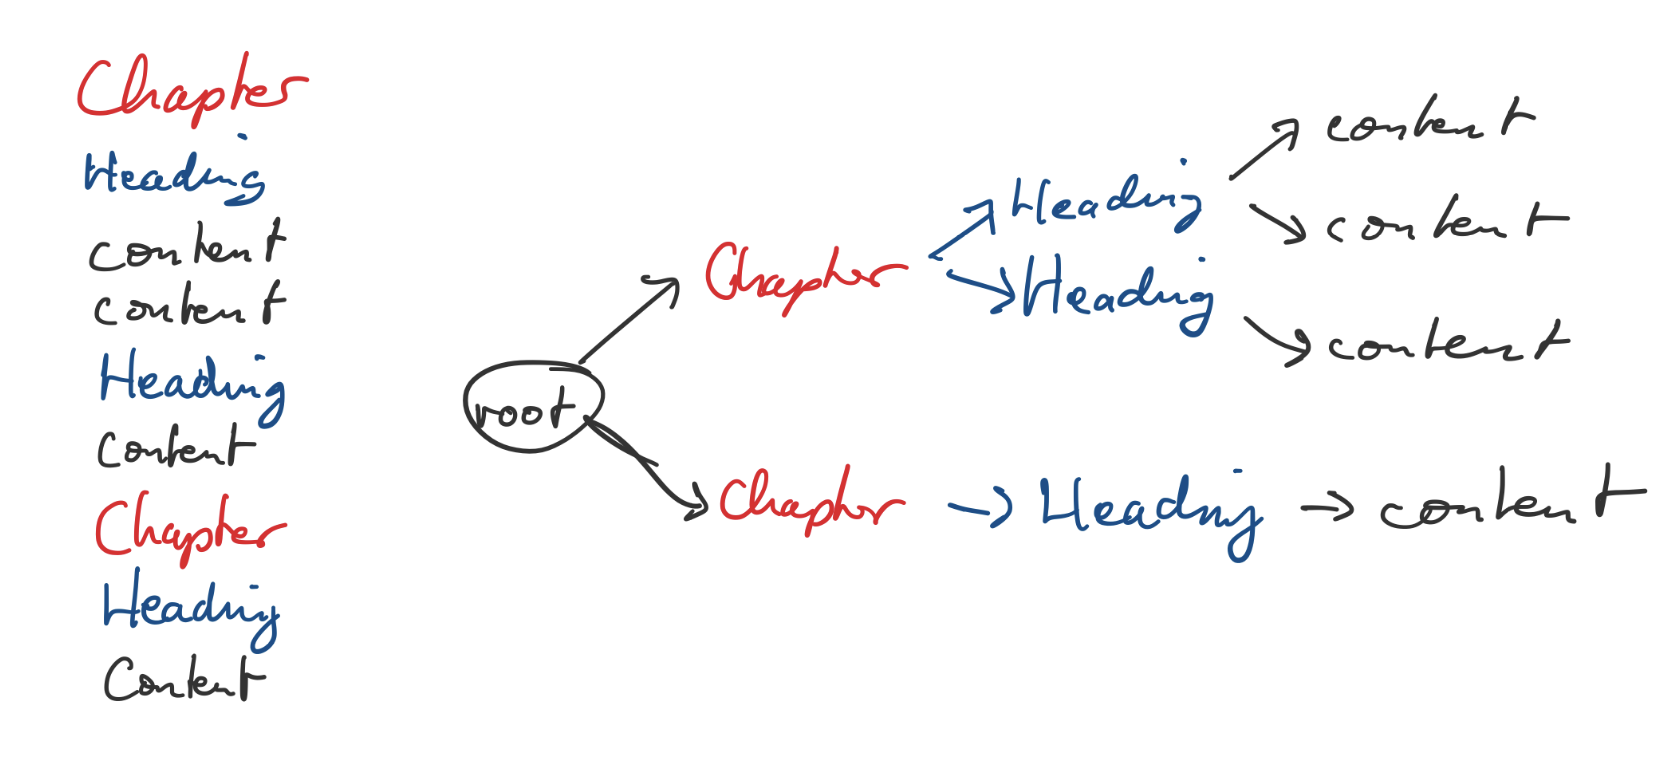
\includegraphics[width=0.8\textwidth]{texttograph}
\caption{representing linear information as text (left) and graph (right)}
\label{fig:treetograph}
\end{figure}

In computer science more powerful ways to store knowledge have been developed. Structured and semi-structured Information is stored with XML, JSON, Databases etc. to great effect. There is no longer a sense of chronology or orientation, but these technologies enable powerful features like querying, search, schemas and transclusion. These advanced Data Models can also be be interpreted as a Graph.

A Graph is thus a very flexible, powerful and interoperable data model for storing information and knowledge. If designed correctly, a graph could leverage the strength of both unstructured text documents and structured database technologies, while serving as the data model for the PKG Ecosystem.

\section{Granularity of Linkable Entities}

An important consideration when talking about data and storage models is the granularity of the data that can be represented. This granularity is essential, because it defines what knowledge can be expressed and associated in a PKG. As outlined in chapter \ref{ch:ecosystem}, we require a data model that is flexible and powerful, able to express atomic and complex concepts and freely associate them.

We investigate the granularity of the smallest entities that different data and storage models allow us to associate with each other. Depending on the context these entities have different names. For files, they are called documents, pages, paragraphs or blocks, for databases they are called rows or cells and for graphs they are called nodes, vertices, entities, or resources.

We will adopt the term knowledge element for the smallest linkable data element in this context \cite{Davies2005Memex60}. In chapter \ref{ch:ecosystem} we have seen, that current PKG tools are based on proprietary formats, most often based on text files or documents. The knowledge elements in this case are documents or pages. 





We will sometimes also refer to these entities as knowledge elements, elements or nodes.

This is the most fundamental consideration. We use the definition  

\section{Data and Storage Models}

% differentiate between data and storage models

% aber viele "Konkurrenten" nutzen doch Textfiles? Kannst ja auch in Text-Files Links definieren (Markup). Was sind die konkreten Stärken und Schwächen - z.B. Performance, Speicherplatzverbrauch, ACID? Finde das folgende mit den Foldern nicht so überzeugend. Beispielsweise speichert mein Wiki die Daten als Textdokumente. Klar kann man darin den Links nicht folgen, wenn ich die mit einem Texteditor öffne, aber das Wiki kann das. Deinen Graphen, wenn der als RDF XML gespeichert wird, kann man das ja auch nicht out-of-the-box, dafür braucht es ne spezielle App. Und letztlich geht’s dabei doch um das Storage, nicht um das Data Model.

% ein Graph ist leicht in einer RDB abbildbar, aber inperformant und umständlich mittels SQL, weil insbesondere rekursive Datensstrukturen nicht unterstützt werden. Auch wieder Storage und nicht Data Model.

% Ist nicht auch Performance ein großer Benefit?

Let us first compare the Storage Models

\textbf{Documents and Files.} While providing excellent orientation and navigation, this approach is too limited. Free association of Knowledge Elements is not possible, as every piece of content belongs to a single Document, and every File belongs to a single folder.

\textbf{relational Databases.} Querying, Freely associationg Knowledge Elements and even Transclusion is possible, but Database Schemata and Management are too restrictive for creating semi- or unstructured Knowledge. The Visualization of Databases also tends to be too complex for non-technical people.

\textbf{Graph Databases.} Graph databases provide the benefits of Relational Databases, while providing intuitive visualizations, flexible schemata and more natural query evaluations for following associated Knowledge.

Many Graph Frameworks could serve as the foundation for the PKG Ecosystem, but the Semantic Web Standards developed by the W3C are especially fitting. As the basis for open Knowledge Graphs and Vocabularies, they have a rich background in Academia and Industry. They provide mature features through Standards like RDF, OWL, SHACL and SPARQL.
Because they are open standards, they are the best bet for PKGs as the basis for lifelong Personal Knowledge Management. 

RDF Knowledge Graphs are **directed labeled graphs.** This Model is also fitting for Personal Knowledge Graphs. Because PKGs are for humans, there is however the additional requirement of making the Data Model human readable. At the very least, all Elements of a PKG need a label.

We will go with a **directed labeled RDF Graph** as the basis for our PKG model. Structured Knowledge will be implemented as closely as possible to Semantic Web Standards. Semi- and unstructured Knowledge will be modeled with Notes using semantic markdown, proposed in chapter [semantic markdown].

\section{RDF Dataset Layers}
% gehts hier um Storage oder Data Model? Temporary Data ist Storage, oder? Adaptive Personal Schema ist Data, oder? Irgendwie fehlt mir da eine Abgrenzung. Ich würde die Aspekte eher separat behandeln. Zumal du ja geschrieben hattest, dass das Backend nicht Teil deiner Thesis sein soll.

The PKG Model consists of a Graph Dataset with several Layers:
\begin{description}
\item[Static external Schema (Ontologies)]Basic Ontologies like RDF, RDFS and OWL will be included by default. Advanced users can add Ontologies and enforce their usage, to make their PKGs mergable with external KGs.

\item[Adaptive personal Schema]The User can freely edit Classes and Properties in his personal Schema, which will be saved for future use.

\item[Structured Data and Notes]This is the main Data Layer of the Personal Knowledge Graph.

\item[Temporary Data]A temporary Data Layer for external RDF Data and runtime generated data gained from Notes, reasoning, inverted links, etc.

\item[Metadata]this data Layer can be used by applications ****to save access rights, order of Notes, or display properties like highlights, alignment, etc.
\end{description}


\section{CRUD operations and effects}

- Quads are RDF Triples with an optional Graph IRI 
(subject, predicate, object, graph?) ~ spog
- Pseudo Code for clarification, a Javascript Implementation can be found in the appendix.
    - Dataset is a triple store / RDF Database
    - function calls are blue and their parameters indented
    - Quads are in Turtle syntax and separated by newlines
    - Each node has an existential triple `node rdf:type rdfs:resource`
    - <IRI> ~ represents dereferencable IRI parameters

\subsection*{Create}

\begin{lstlisting}
// create Class "Idea" (into users personal schema layer)
// inserts the quads in this array into the dataset
Dataset.addQuads
  :IRI rdf:type rdfs:Resource :UserSchema
  :IRI rdf:type rdfs:Class :UserSchema
  :IRI rdfs:label "Idea" :UserSchema
\end{lstlisting}

\begin{lstlisting}
// create Relationship "author" (into users personal schema layer)
Dataset.addQuads
  :IRI rdf:type rdfs:Resource :UserSchema
  :IRI rdf:type rdfs:Property :UserSchema
  :IRI rdfs:domain rdfs:Resource :UserSchema
  :IRI rdf:range rdfs:Resource :UserSchema
  :IRI rdfs:label "author" :UserSchema    
\end{lstlisting}

\begin{lstlisting}
// create Node "Hypothesis" (into data layer)
Dataset.addQuads
    :IRI rdf:type rdfs:Resource :Data
    :IRI rdfs:label "Hypothesis" :Data

\end{lstlisting}

\subsection*{Read}  

\begin{lstlisting}
// get Quad with matching subject, predicate, object, graph 
// returns: Array of matching Quads
Dataset.match
  subject 
  predicate
  object
  graph
\end{lstlisting}




\begin{lstlisting}
// get Quads with matching subject and wildcards for  predicate, object, graph
Dataset.match
  subject      //e.g. :IRI or Literal "Hypothesis"
  * 
  *
  *

\end{lstlisting}


\subsection*{Delete}  

\begin{lstlisting}
// delete Class or Node <:IRI>
// deletes all quads that include this node
Dataset.deleteQuads
  Dataset.match
    <:IRI> 
    * 
    * 
    *
Dataset.deleteQuads
  Dataset.match
    * 
    <:IRI> 
    * 
    *
Dataset.deleteQuads
  Dataset.match
    * 
    * 
    <:IRI> 
    *

\end{lstlisting}
\begin{lstlisting}
// delete Relationship <:IRI>
// deletes all quads that include this relationship
Dataset.deleteQuads
  Dataset.match
    * 
    <:IRI> 
    * 
    *

\end{lstlisting}

\begin{lstlisting}
// delete Quad s p o g
// deletes this quad
Dataset.delete
  s
  p
  o
  g

\end{lstlisting}

\subsection*{Update} 
can be implemented either as a combination of delete and create operations or as more performant in-place operations. The in-place operations need to be optimized for performance, based on the exact tech stack.

\begin{lstlisting}
// update Label to "Hypothesis"
Dataset.deleteQuads
  Dataset.match
    <:IRI> 
    rdfs:label 
    * 
    *

Dataset.addQuads
  :IRI rdf:type rdfs:Resource :Data
  :IRI rdfs:label "Hypothesis" :Data

\end{lstlisting}

% \section{Advanced Semantics with OWL?}

\section{Markdown Outliner in RDF}

% insert a diagram of transclusion and order of text nodes.
In this section I propose an implementation for storing semistructured Text in RDF.

Note that because RDF Graphs are unordered, Text nodes need to be coupled with metadata defining display order, etc.

Let us start with a simple example:

\begin{lstlisting}
:IRI rdf:type :Person, :Artist, :Musician
:IRI rdfs:label "Lady Gaga"
:IRI foaf:givenName "Stefani Joanne Angelina"
:IRI foaf:familyName "Germanotta"

\# attaches the note to <:IRI> Lady Gaga entity
:IRI :note :note\_000                
:note\_000 rdf:type :SemanticMarkdown
:note\_000 rdfs:label "Here is some Trivia about Lady Gaga:"
:note\_000 :note :note\_001
:note\_001 rdf:type :SemanticMarkdown
:note\_001 rdfs:label "Lady Gaga is not her real name."
:note\_000 :note :note\_002
:note\_002 rdf:type :SemanticMarkdown
:note\_002 rdfs:label "She is sometimes confused with [Gwen Stefani]"
:note\_000 :note :note\_003
:note\_003 rdf:type :SemanticMarkdown
:note\_003 rdfs:label "She got a lot of attention for extravagant dresses, 
    like her [Meat Dress]"
\end{lstlisting}


Could be rendered like this by a PKG Tool:

\begin{lstlisting}
- rdfs:label -> "Lady Gaga"
- rdfs:type -> [Person], [Artist], [Musician]
- foaf:givenName -> "Stefani Joanne Angelina"
- foaf:familyName -> "Germanotta"

- Here is some Trivia about Lady Gaga:
    - Lady Gaga is not her real name.
    - She is sometimes confused with [Gwen Stefani]
    - She got a lot of attention for extravagant dresses, like her [Meat Dress]
\end{lstlisting}


The RDF Property `:note` is special and signals to the PKG Tool that this Entity should be treated as a Text Note / Semantic Markdown on the Entity. Note that all of the unstructured text notes are still their own IRIs. This means SemanticMarkdown can be associated with or rendered on an unlimited number of other Entities. They have `rdf:type :SemanticMarkdown` , which signals the PKG Tool to render it in outliner mode.

\begin{figure}[H]
    \includegraphics[width=0.5\textwidth]{pkg}
\end{figure}

% - ~~simply "taking notes" in English text involves no learning curve such as that required for creating alien graphical diagrams. (blödsinn, wir lernen lesen nur in der Schule)~~

% - It is worth mentioning that

% 1.  lots of people are not satisfied with SWS and even the creators acknowledge Problems in design (better rdf repo) and

% 2.  standards can change and be extended (RDF*) thus the basis for the model is graph theory, not SWS theory. For now the selected graph model will be RDF

% When **loading RDF into a human readable editor, you get a load of machine relevant meta crap**